
    \subsection*{Distance from the Origin to the Plane}
    
        \begin{figure}[H]
            \centering
                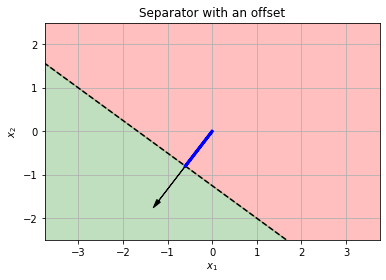
\includegraphics[width=70mm,scale=0.5]{images/classification_images/separator_with_offset_shown.png}
                \caption*{Notice that the \textbf{shortest} path from the origin to the line is \textbf{parallel} to $\theta$!}
        \end{figure}
        
        So, we can think of our \textbf{line} as having been \textbf{pushed} in the $\theta$ direction. This \textbf{matches} what we did for 1-D separators: $x_1>3$ was moved in the $x_1$ direction.
        
        So, we'll take the closest point on the line, $\vec{d}$. The \textbf{magnitude} $d$ will give us the \textbf{distance} that the separator has been \textbf{shifted}.
        
        \begin{figure}[H]
            \centering
                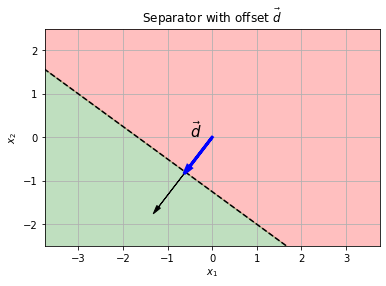
\includegraphics[width=70mm,scale=0.5]{images/classification_images/separator_with_offset_d.png}
        \end{figure}
        
        Since $\vec{d}$ is in the direction of $\theta$, the direction can be captured by the unit vector $\hat{\theta}$. Let's take a look at that:
            \note{Remember, a vector is direction (unit vector) times magnitude (scalar).}
            
        \begin{equation}
            \theta = \norm{\theta} \red{\hat{\theta}}
        \end{equation}
        
        \begin{equation*}
            \vec{d} = d \red{\hat{\theta}}
        \end{equation*}
        
        $\vec{d}$ is on the \textbf{line}, so it satisfies:
        
        \begin{equation}
            \theta^T \vec{d} + \theta_0=0
        \end{equation}
        
        Since $\theta$ and $\vec{d}$ are in the same direction, we can use that fact:
        
        \begin{equation}
            \norm{\theta} 
            \red{\hat{\theta}} \cdot d \red{\hat{\theta}}
            + \theta_0
            = 
            \norm{\theta} \left( 
                                \red{\hat{\theta} \cdot \hat{\theta}} 
                          \right) 
                          d + \theta_0
        \end{equation}
        
        We know that $\hat{u} \cdot \hat{u}=1$:
        
        \begin{equation}
            \norm{\theta}d+\theta_0=0
        \end{equation}
        
        And now, we just solve for $d$:\\
        
        \begin{concept}
            The \vocab{distance} $d$ from the \purp{origin} to our \gren{linear separator} is 
            
            \begin{equation}
                d = \frac{ -\theta_0}{\norm{\theta}}
            \end{equation}
        \end{concept}
        
        A "negative" distance means $\vec{d}$ (the vector from the origin to the line) is pointed in the opposite direction of $\theta$.
        
        \begin{figure}[H]
            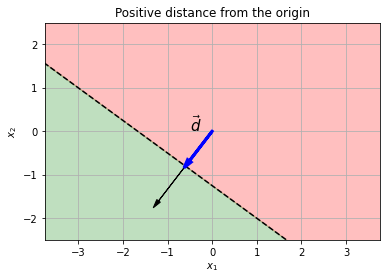
\includegraphics[width=70mm,scale=0.5]{images/classification_images/positive_distance.png}
            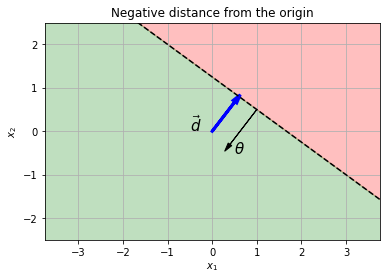
\includegraphics[width=70mm,scale=0.5]{images/classification_images/negative_distance.png}
            
        \end{figure}
        
        Notice, again, that this agrees with our \textbf{earlier} thought: the sign of $\theta_0$ is the opposite ($-1$) of the $\theta$ direction we move in.